\chapter[The pSeg plasmid library]{pSeg: plasmids for live-cell segmentation}
\label{pseg}

This dissertation uses only fixed-cell microscopy
assays, but future studies would ideally include
live-cell studies of \tgfbsf\ and Wnt signaling.
Live-imaging and fixed-cell imaging can use the same
general analytical methods,
including the use of nuclear and cytosolic fluorescence
to identify these two cellular compartments. However,
finding appropriate labels for live-cell assays is much more difficult,
as the cells are not permeabilized and toxic stains must
be avoided. In order to effectively deploy segmentation
algorithms, the nucleus and cytosol should ideally be labeled
brightly and homogeneously.


 \begin{figure}[!b]
  \centering
  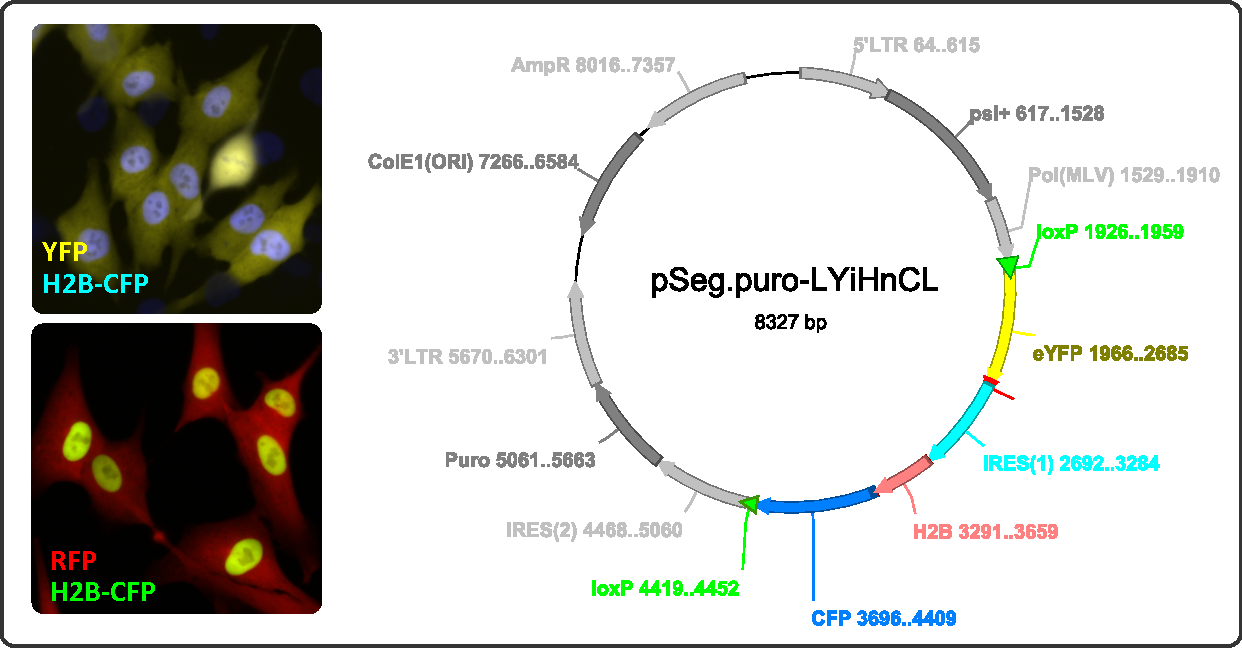
\includegraphics[width=6in]{FIGS/pseg/structure.pdf}
  {\singlespacing 
  \caption[ pSeg structure and sample images.]
            { The pSeg plasmids generally consist of two
            differentially-localized fluorophores. Left, sample
            images from two human colonic
            epithelial cell (HCEC) pSeg clones. The top image is from
            the LYiHnCL pSeg construct shown at right,
            and the bottom image is from an LRiHnCL construct.
            See \ar{table:pseg:symbols} for symbols.
            Right, structure of pSeg construct. The 5' and
            3' Murine Leukemia Virus LTRs
            (long terminal repeats) flank the
            construct, which also has loxP sites oriented
            in the same direction so that the construct
            can be excised by Cre recombinase, thus reverting
            a clone to a ``parental'' phenotype. AmpR, ampicillin
            resistance gene. psi+, viral packaging sequences. Puro,
            puromycin. IRES, internal ribosome entry site.}
  \label{fig:pseg:structure}}
  \end{figure}

One approach to address this problem is via ``central dogma'' (CD)
tagging, in which a fluorescent-protein-encoding gene surrounded by
splice acceptor/donor sites is randomly integrated
into the genome. Any integration that lands within an intron of a gene
has a chance to become an exon for that same gene. Thus,the genetic protein
product will then contain a fluorescent protein as one of its domains,
allowing the localization and dynamics of that protein to be visualized
\cite{Jarvik1996,Jarvik2002}.


High-throughput studies have used this technique to obtain
nucleus- or cytosol-localized labels for the purpose of segmentation,
with the purported benefit that it requires no exogenous expression system
and thus minimizes perturbations to the cell
\cite{Sigal2006,Sigal2007,Sigal2006a,Issaeva2010}. Unfortunately,
the CD-tagging process is slow, since exon-generating integration
events are rare and must be subsequently screened to identify
the rarer-still events that yield the desired localization patterns.
Additionally, the tagging of a protein is itself a perturbation that
may disrupt localization or function. Chosen CD-tagged clones must
then be carefully studied to ensure that the cells (and the tagged
proteins) behave properly.


A much faster alternative is to express
fluorescent proteins from exogenous promoters, though there is
always the concern that the presence of an exogenous promoter may
affect the cell in some unpredictable way. To me, this
is just as problematic as the concern that CD-tagging will
disrupt some unknown function of the tagged protein.
I therefore prefer the efficiency of the exogenous approach.
To take advantage of this efficiency for future live-cell projects, I
created a library of viral constructs, each generating distinct
localization patterns of red, yellow, and cyan fluorescent
protein expression in mammalian cells. I refer to these
as ``segmentation plasmids'' (pSegs).


    \begin{table}[!bt]
    \centering
	\footnotesize
    \caption[List symbols for the pSeg library.]
    { List symbols for the pSeg library in \ar{table:pseg:library}.}
    \label{table:pseg:symbols}
    \begin{tabular}{cll}
    \hline
    Symbol   & Abbreviation & Full \\ \hline
    C & CFP  & mCerulean\\
    G & GFP  & enhanced Green Fluorescent Protein\\
    H & H2B  & Histone H2B (\fly)\\
    i & IRES & Internal ribosome entry site (encephalomyocarditis virus)\\
    L & loxP & loxP site \\
    n & NLS  & Nuclear Localization Signal (SV40)\\
    m &      & membrane- localized Gap43 N-terminus (\i{Danio rerio})\\
    R & RFP  & mCherry\\
    Y & YFP  & enhanced Yellow Fluorescent Protein\\
    \hline
    \end{tabular}
    \end{table}



\subsubsection{pSeg structure}


Each pSeg plasmid has three variable components:
a fluorescent protein (FP) with a whole-cell expression
pattern, a fluorescent protein with a nuclear
expression pattern, and a selection cassette.
I chose the mCherry, eYFP, and Cerulean fluorescent proteins
because they have wide spectral separation and so can all
be used simultaneously in single cells.
The general structure of the insert is
shown in \ar{fig:pseg:structure}.
Whole-cell expression patterns are generated by either
free FP or a FP fused to the Gap43 membrane localization
signal \cite{Livet2007}.
This signal results in faint whole-cell and strong
membrane fluorescence.
Nuclear expression is mediated by addition of either a
nuclear localization sequence (NLS) or fusion to \fly\ histone H2B.
The H2B-fused FP is useful because it can be used to
monitor chromatin condensation \cite{Snippert2011} and
seems to be benign even when generally expressed in mice
\cite{Neurohr2009}.

   \begin{table}[!bt]
    \centering
	\footnotesize
    \caption[List of pSeg plasmids.]
    { Full list of plasmids in the pSeg library. See
     \ar{table:pseg:symbols} for symbol meanings. ``Floxed''
     refers to flanking by loxP.
     PuroR and NeoR refer to puromycin or neomycin resistance
     cassettes.}
    \label{table:pseg:library}
    \begin{tabular}{lll}
    \hline
    floxed \& PuroR & floxed \& NeoR & NeoR   \\ \hline
    LmYiHnCL        & LYiHnCL        & YiHnC  \\
    LmCiHnCL        & LGiHnCL        & YiHnY  \\
    LmRiHnCL        & LRiHnCL        & CiHnC  \\
    LmYiCnnCL       & LYiCnnCL       & CiHnY  \\
    LmCiCnnCL       & LGiCnnCL       & YiCnnC \\
    LmRiCnnCL       & LRiCnnCL       & YiYnnY \\
    LYiHnCL         &                & CiCnnC \\
    LGiHnCL         &                &        \\
    LRiHnCL         &                &        \\
    LYiCnnCL        &                &        \\
    LGiCnnCL        &                &        \\
    LRiCnnCL        &                &        \\ \hline
    \end{tabular}
    \end{table}


Each construct is expressed as a single
mRNA, using the retroviral promoter and an internal
ribosome entry site (IRES) for differential translation
of the the protein products. Finally, the constructs are
also flanked by loxP sites and so can be removed after
genomic integration, thus generating unlabeled ``parental'' cell lines.
The pSeg library consists of 25 color/localization/selection 
combinations in Puromycin or Neomycin-resistant backgrounds,
with or without flanking loxP sites.
\ar{table:pseg:library} shows all of
these constructs (refer to \ar{table:pseg:symbols} for symbol definitions).


I built the library into
the pMYs retroviral backbone, which contains a modified
version of the Murine Leukemia Virus promoter that
improves integration efficiency in some stem cell systems \cite{Kitamura2003}.
The pMYs backbone contains the viral long terminal repeats
(LTRs) and a viral packaging signal (\ar{table:pseg:symbols}), allowing for the creation
of virus using MLV packaging cell lines. 


\subsubsection{Generating cellular pSeg clones}


Integration of the pSeg constructs into target
cells requires the generation of and infection by
live virus (see \nameref{pseg:methods}). A few days
after infection, I FACS (Flow-assisted cell sorting)-sort
single cells into each well of 384-well
plates. I find that survival rates
for singly sorted cells are quite low ($\sim$20-30\%), though
I could double these rates by pre-seeding the
wells with un-labeled cells. The feeder cells can
be selected against later according to the chosen pSeg cassette.
With this appraoch, a clone from the A549 cell line was created in the
Altschuler \& Wu lab by Jungseog Kang and Qi Wu, which
forms the foundation of a CD-tagged library (unpublished).


The slowest part of the process is the establishment of clonal
cell lines from single cells, which can take 6 weeks.
However, this step is essential.
Cell-to-cell variability can be high, even within
a clonal population \cite{Singh2010}. Further, I found that all
pSegs yield populations with diverse localization patterns.
For example, the LRiHnCL construct should express
mCherry and Cerulean in the nucleus, and yet all
possible patterns are observed (\ar{fig:pseg:mixed}).
The reason for this is not clear, though retroviruses
(such as MLV) have diploid genomes within viral
particles and are known to have recombination events
\cite{Coffin1997}. The high degree of repetition within
these constructs (the different fluorescent proteins
have high homology) may then lead to truncations or
expansions of the integrated sequence, such that it
re-arranges the localization signals on the fluorescent
proteins.


Finally, I warn that the Murine Leukemia Virus has
a strong preference for integration into the 5' end
of highly-expressed genes
\cite{Wu2003a,Mitchell2004,Cattoglio2010}. Despite this
preference, the virus does seem to
avoid house-keeping genes, though I note that this
may simply be due to the death of cells that do have
integrations at such sites. As a consequence of integration,
then, functionally important genes may be disrupted. A simple test for
this is to select multiple labeled clones and compete each
against the unlabeled parental population. The clones with the
most similar-to-parental growth rates can then be kept for further experiments. 


 \begin{figure}[tb]
  \centering
  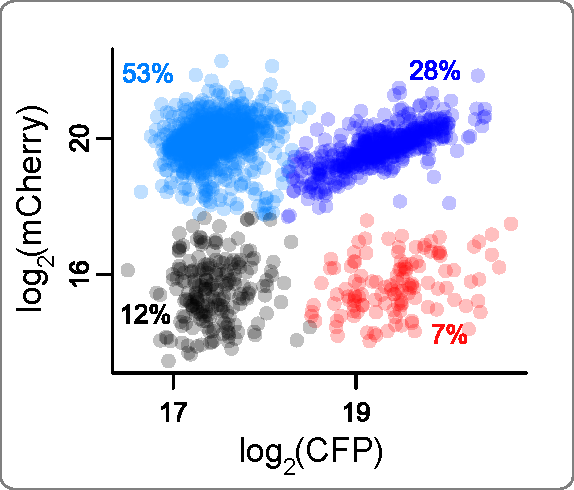
\includegraphics[width=3in]{FIGS/pseg/mixed.pdf}
  {\singlespacing 
  \caption[ Requirement for pSeg clonal selection.]
            { A population of cells infected with the
              pSeg.puro-LRiHnCL construct show all possible
              nuclear localization patterns. Percents show
              the relative population size for each group.
              The bottom-left (black) cells are unlabeled,
              the top-right (dark blue) cells are correctly
              labeled with both fluorescent proteins, and
              the other two populations express only one
              of the two proteins. $n$=1770 human colonic
              epithelial cells, stained with Hoechst for
              segmentation. Arbitrary total fluorescence units.}
  \label{fig:pseg:mixed}}
  \end{figure}






\subsubsection{Methods}
\label{pseg:methods}

\b{Molecular cloning.}
I constructed the pSeg library using a combination 
of standard moleculuar cloning techniques and 
Gibson assembly (New England Biolabs \#E5510)
\cite{Gibson2010}. I verified each construct
by Sanger sequencing, and confirmed each phenotype
by checking the localization patterns in 
transiently-transfected HEK293T cells.


\b{Tissue culture.}
The tissue culture methods and imaging followed those
in \ar{insulation:methods} with the exception of
viral production and infection.
I used the Platinum-A HEK293T packaging
cell line (Cell Biolabs \#RV-102)
and closely followed the protocol used by Uri Alon's
group for CD-tagging \cite{Sigal2007}. 
In brief, virus is generated by transfecting packaging
cells and collecting the supernatant 2-3 days later. This
supernatant is then applied to the target cells, which
are left for 48-72 hours to allow for genomic integration. The
multi-day timeline is essential, as MLV can only
integrate into immediately-post-mitotic
genomes \cite{Roe1993}.


\b{Analysis.}
For the analysis in \ar{fig:pseg:mixed} I used the ImageJ
implementation of the rolling ball algorithm for
correction and a custom Matlab nuclear threshold segmentation algorithm.
I used the Hoechst channel
to manually gate the G1 population and to subsequently
correct the mCherry and Cerulean channels using the
regression method described in
\ar{imaging:singleCellCorrection}. I used
the k-means algorithm implemented in R to automatically
identify each of the subpopulations shown in the figure.

